\chapter{Calcium Waves from RyR}
\label{chap:calcium_waves_RYR}


\section{Introduction}

The link between $\Ca$ sparks and waves have been documented before
\citep{cheng1996csc,wier1997, lukyanenko1999}. However, it's not well known how
or under which condition a $\Ca$ spark can initiate a wave, while the others
cannot. At the tissue level, the wave need synchronized activation from multiple
cells at the same time. Similarly, at the cellular level, the wave need
synchronized activation from multiple CRUs. However, by random displacement of
CRUs, and the independency between these CRUs, the wave frequency would be much
lower than that observed in experiments. To resolve this question, there should
be some mechanism that link CRUs leading to self-organization of $\Ca$ spark
clusters. 

Calcium sparks amplitude and spread are known to increase during calcium
overload conditions, which favor the initiation of calcium waves
\citep{cheng1996csc}. Saltatory propagation characteristics of $\Ca$ wave refer
the property that the front of the wave jumps from one release site to
another \citep{keizer1998}. There are different types of waves, e.g.
semi-circular, circular and spiral waves with propagation velocities from
30$\mum/s$ to 150$\mum/s$ were observed \citep{engel1994apc, takamatsu1990,
wussling1996}.

\citep{nivala2012} proposed a theoretical framework in which (1) the
cluster-size distribution is exponential when the coupling between CRU is week,
(2) the distribution is power-law when the coupling between CRUs become strong
(Sect.\ref{sec:nivala2012}). So, a power-law distribution is an indicator that
the system is in critical state.

Cardiac cells were shown to develope spatio-temporal calcium patterns:
oscillation \citep{wier1991}, circular \citep{williams1992, takamatsu1990} or
spiral waves \citep{lipp1993} (review: \citep{wussling1999}).

\subsection{Mechanism of $\Ca$ waves}

In Purkinje fibres, \citep{wier2000} observed that electrical stimulation
elicited an AP, leading to the increase in fluoresence concentration (L0)
compared to resting levels (accounted by the inward calcium via LCC). 
\begin{itemize}
  \item Average intensity increase of L0 over resting value was about 63\%,
  which suggest free $[\Ca]_i$ increase from 0.1$\muM$ to 0.2$\muM$ (as derived
  from the back calculation \citep{cheng1993cse})
\end{itemize}
In about 38\%, this was followed by a further increase of fluorescence along the
edges of the cell (L1) which is accounted by the release of calcium from corbular SR. The
direction of L1 traveled from long edges of the cell toward the core of the
cells. 

In 62\% of the paced tests, L0 is followed by some focally arising of $[\Ca]$
(known as L2), e.g. 2 different foci, each focus gives rise to a $\Ca$ waves
propagatin along the cell. The waves from different foci can travel at opposite direction. At the
site of the collision, reuptake occurs, and the wave is abolished. 

In some situation, focally arising $\Ca$ waves (known as L2*) can also occur
without any electrical stimulation (i.e. no L0). This spontaneous $\Ca$ waves
appeared to originate from the cell borders and propagate longitudinally with
velocity $V_{prop}=164\pm 10 \mum$/s \citep{wier2000}. About 28\% of such
situations, this wave L2* can trigger L0, and eventually leading to L1. This
suggest that spontaneous $\Ca$ waves can depolarize sufficient the membrane
potential to cause AP. This spontaneous AP of course trigger L0 and L1 like 
stimulated AP. 

The mechanism for $\Ca$ ions moving from peripheral subsarcolemmal area to the
cell core was accounted by 2 hypothesises: (1) $\Ca$ diffusion
\citep{spitzer1997}, (2) CICR (via corbular SR) in combination with diffusion
\citep{wier2000}. Also, the $\Ca$ waves and membrane depolarizations are
sensitive to thapsigargin, a drug that block SERCA leading to low $\Ca$
re-uptake back to SR. So, the level of SR $\Ca$ plays a significant role in
triggering calcium waves. 

\subsection{Measure $\Ca$ waves}
\label{sec:measure_Ca-wave_RYR}

To see how $\Ca$ waves were measured from IP3R-mediated waves, read
Sect.\ref{sec:measure_Ca-wave_IP3R}.
 
\citep{wier2000} determined the parameters of movement of $\Ca$ waves from light
intensity profiles of the processed fluorescence images. Upward deflections
indicate fluorescence changes corresponding to a local increase in intracellular
$[\Ca]_i$. Wave velocity was calculated from positions of $\Ca$ transient over
time from the steepest midportion of the transient. Only $\Ca$ along the
longitudinal direction was calculated. $\Ca$ waves propagated along the
transverse direction was ignored in the analysis.




\section{Fire-diffuse-fire models}

Early models used the fire-diffuse-fire approach in modelling calcium waves
\citep{bugrim1997, keizer1998, izu2001, subramanian2001}. The models focused on
diffusion-coupled calcium-induced calcium release, with properties like release
site spacing, non-uniformity in spatial distribution of release sites,
sensitivity of RyR channels, the role of jSR calcium, and SERCA pumps.

\section{Blackx et al. (1989) - $\Ca$ waves}
\label{sec:blackx-et-al}

~\cite{backx1989} proposed the first deterministic, one-dimensional
model of $\Ca$ waves.

The propagated spontaneous contraction observed in the cardiac cell was not
related to CICR, but to release as a consequence of $\Ca$ overload
\citep{fabiato1985scc}. This spontaneous contraction has a profound effect on
force generation. However, provided that the frequency of spontaneous
contraction is lower than the rate of stimulation of the preparation, the force
generation won't be affected. Nevertheless, the frequency of oscillations and
velocity of propagation are influenced by condition and chemical agents, e.g.
caffeine, ryanodine, verapamil, procaine, \ldots.

To study calcium oscillation, \citep{backx1989} developed a simple model of CICR
and calcium diffusion, i.e. $\Ca$ is released from SR, diffusing into the
adjacent cytosol, thereby inducing calcium release.

The release from SR occur when $[\Ca]$ reaches a threshold, e.g. 1.2$\muM$. The
release function was described as an exponential rise and fall of $\Ca$ flux
from SR, with 2 first-order gating variables: on e activation and one
inactivation. $\Ca$ is sequestered back to SR via SERCA. 

Under 1D model, the finite difference method is used \citep{cannell1984,
crank1975}. With $N$ grid point, each grid point contains 7 variables.
\begin{equation}
\begin{split}
d[\ca]/dt = \\ 
d[\CaM]/dt  = \\
d[
\end{split}
\end{equation}
with the order $[\Ca]$, unbound calmodulin (CaM), 

The boundary condition is $d[\ca]/dt_{x=\{O,L\}}=0$, i.e. the calcium doesn't
pass at either end O and L.  

Rate constants of $\Ca$ binding to troponin and calmodulin was derived from
\citep{robertson1981, potter1981}. $[\Trpn]$ and $[\CaM]$ were derived from
\citep{wier1986}.

The diffusion constant of $\Ca$: $D_\ca = 400 \mum^2/s$. NOTE: The diffusion
constant of pure water is $700 \mum^2/s$ \citep{wang1953}. However, due to
intracellular milieu has an ionic strength of 0.17, and the presence of other
proteins, the diffusion constant of calcium in the cell is lower than in pure
water. The diffusion constants was also assumed to be homogeneous throughout the
length of the cell.

 The numerical method: 6th-order predictor-corrector methdo with a
variable step size \citep{gear1971}.

With 100 grid points per sarcomere, and they simulated 20-500 sarcomeres with 10
release sites.



\section{Lipp et al. (1993) - Spiral waves}

\citep{lipp1993}


\section{Skupin et al. (2008) }

\citep{skupin2008}

\section{Restrepo-Weiss-Karma (2008)}
\label{sec:restrepo-weiss-karma}

This model was created to test the hypothesis that the delay in CSQN
binding/unbinding can cause calcium transient alternans
(CTA)~\citep{restrepo2008cmm}, regardless of \ce{Ca^2+} load
alternating. 
% As the {\it local control theory} is widely accepted,
% i.e. the elementary \ce{Ca^2+} release events are \ce{Ca^2} sparks,
% whole-cell \ce{Ca^2+} signals is the summation of all these \ce{Ca^2+}
% sparks. Each site for \ce{Ca^2+} spark is called \ce{Ca^2+} release
% unit (CRU); or stochastic functional unit (SFU) due to the fact that
% the \ce{Ca^2+} spark events are stochastic.

\subsection{Cell structure} 

\textcolor{red}{This model investigate the submembrane space as well}. The
magnitude of the current in each submembrane space is determined by the number
of NCX per unit, and was chosen so that the whole-cell NCX current is
physiological. The 3D distribution of CRUs is discussed in
Sect.\ref{sec:cru_calcium_release_unit}. Here, the model use $l_T=0.9\mu$m
(transverse separation), and $l_L=1.84\mu$m (longitudinal separation). Based on
the myocyte shape aspect ratio given by ~\citep{satoh1996svr}
\begin{equation}
  \label{eq:870}
  140\mu m \times 30 \mu m \times 12 \mu m
\end{equation}
$V_\text{cell}\approx 30$ (pL) and the number of CRUs in each dimension was
given as $n_x=65, n_y=27, n_z = 11$; thus given the total number of CRUs as
$N=19,305$.  In this model, the effective cytosolic volume $V_{cyto}=10$pl
(\textcolor{red}{quite small compared to experimental data of 18pL}). 

NOTE: the proximal space here means the dyadic subspace.

\subsection{CRU model}

\begin{figure}[hbt]
  \centerline{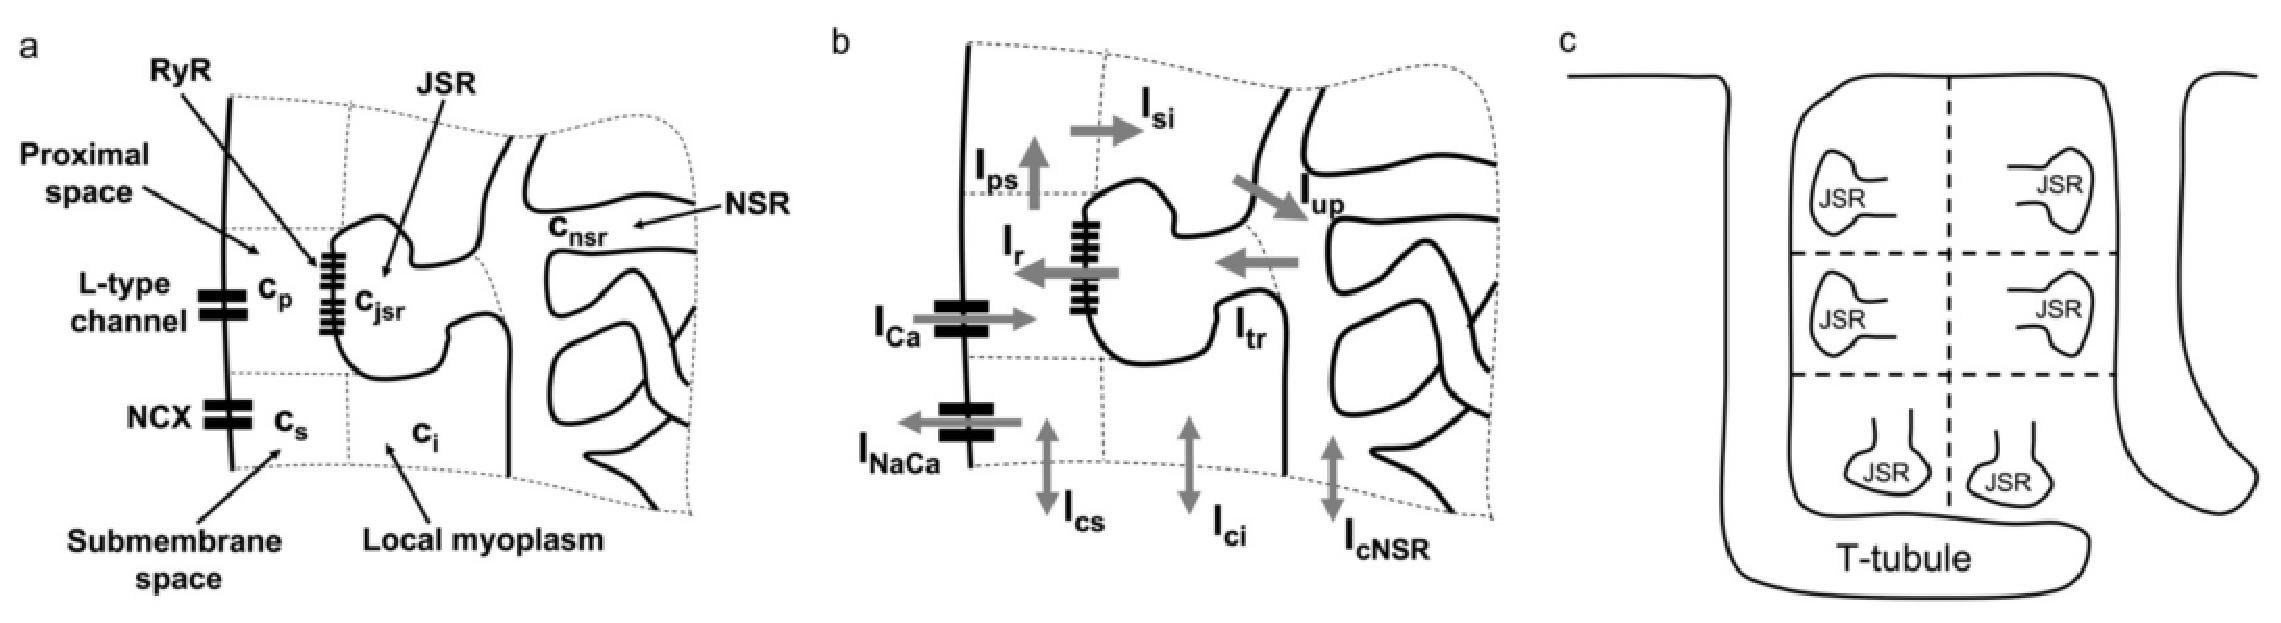
\includegraphics[height=3cm,
    angle=0]{./images/restrepo_CRU.eps}}
  \caption{(a) a CRU with local cytosolic (myplasm) $V_i$, submembrane $V_p$,
    proximal space $V_p$, JSR $V_\jsr$, NSR compartment $V_\nsr$; (b) The fluxes
    and the ionic currents - $I_{Ca}$ at proximal space and $I_{NCX}$ at submembrane
    space; (c) schematic illustration of the heterogeneous orientation
  of the T-tubule inside the myocyte}
\label{fig:restrepo_CRU}
\end{figure}

Each release is modeled with 5 sub-compartments, each with its own volume as
shown in Fig.\ref{fig:restrepo_CRU}. The five local volumes inside a CRU
of index $n$ are
\begin{equation}
  \label{eq:871}
  \begin{split}
    V_i^{(n)} &= 0.5\mu m^3 \\
    V_s^{(n)} &= 0.025\mu m^3 \\
    V_{JSR}^{(n)} &= 2\times 10^{-2} = 0.02\mu m^3 \\
    V_{NSR}^{(n)} &= 0.025\mu m^3 \\
  \end{split}
\end{equation}
NOTE: they assumed
\begin{equation}
  \label{eq:872}
  V_i^{(n)} = V_{cyto}/N = 20 V_s^{(n)} = 20V_{NSR}^{(n)}
\end{equation}


Realistically, the number of RyRs per CRU, the number of LCC per CRU should have
random variation. \textcolor{red}{However, for simplicity, it is assumed that
all CRUs have the same number of LCCs and RyRs}.
Given that the more number of LCCs per CRU; the more heterogeneous $I_\LCC$
current amplitude per CRU. To replicate this phenomenon, instead of using high
number of LCCs; this model use only 4 LCCs per CRU and varies the proximal space
volume, which change the \ce{Ca^2+} concentration and indirectly affect the
$I_\LCC$. \textcolor{red}{Given the using of 100 RyRs and 4 LCCs per CRU. This
is somewhat move away from the proper ratio 1/4 to 1/10 for LCC:RYR}.

The variation in the proximal space is given by
\begin{equation}
  \label{eq:873}
  V_p^{(n)} = 1.26\times 10^{-3}\mu m^3 \times (1+r^{(n)})
\end{equation}
with $r^{(n)}$ is a random  number drawn from Gaussian distribution with
mean 0 and standard deviation 0.3; truncated to restrict $r^{(n)}$ in the
interval $[-0.8, 0.8]$. This number is chosen at the beginning of the
simulation and doesn't change during the whole simulation. The average
proximal space is 0.00126$\mum$ as a cylindrical space of radius
$200$nm and height $10$nm~\citep{hinch2004mag}.

\subsubsection{RyR model}

4-state Markov model with CSQN server as $\Ca$ sensor to regular the gating
(Sect.\ref{sec:RYR_Restrepo2008-CSQ}).

% \begin{figure}[hbt]
%   \centerline{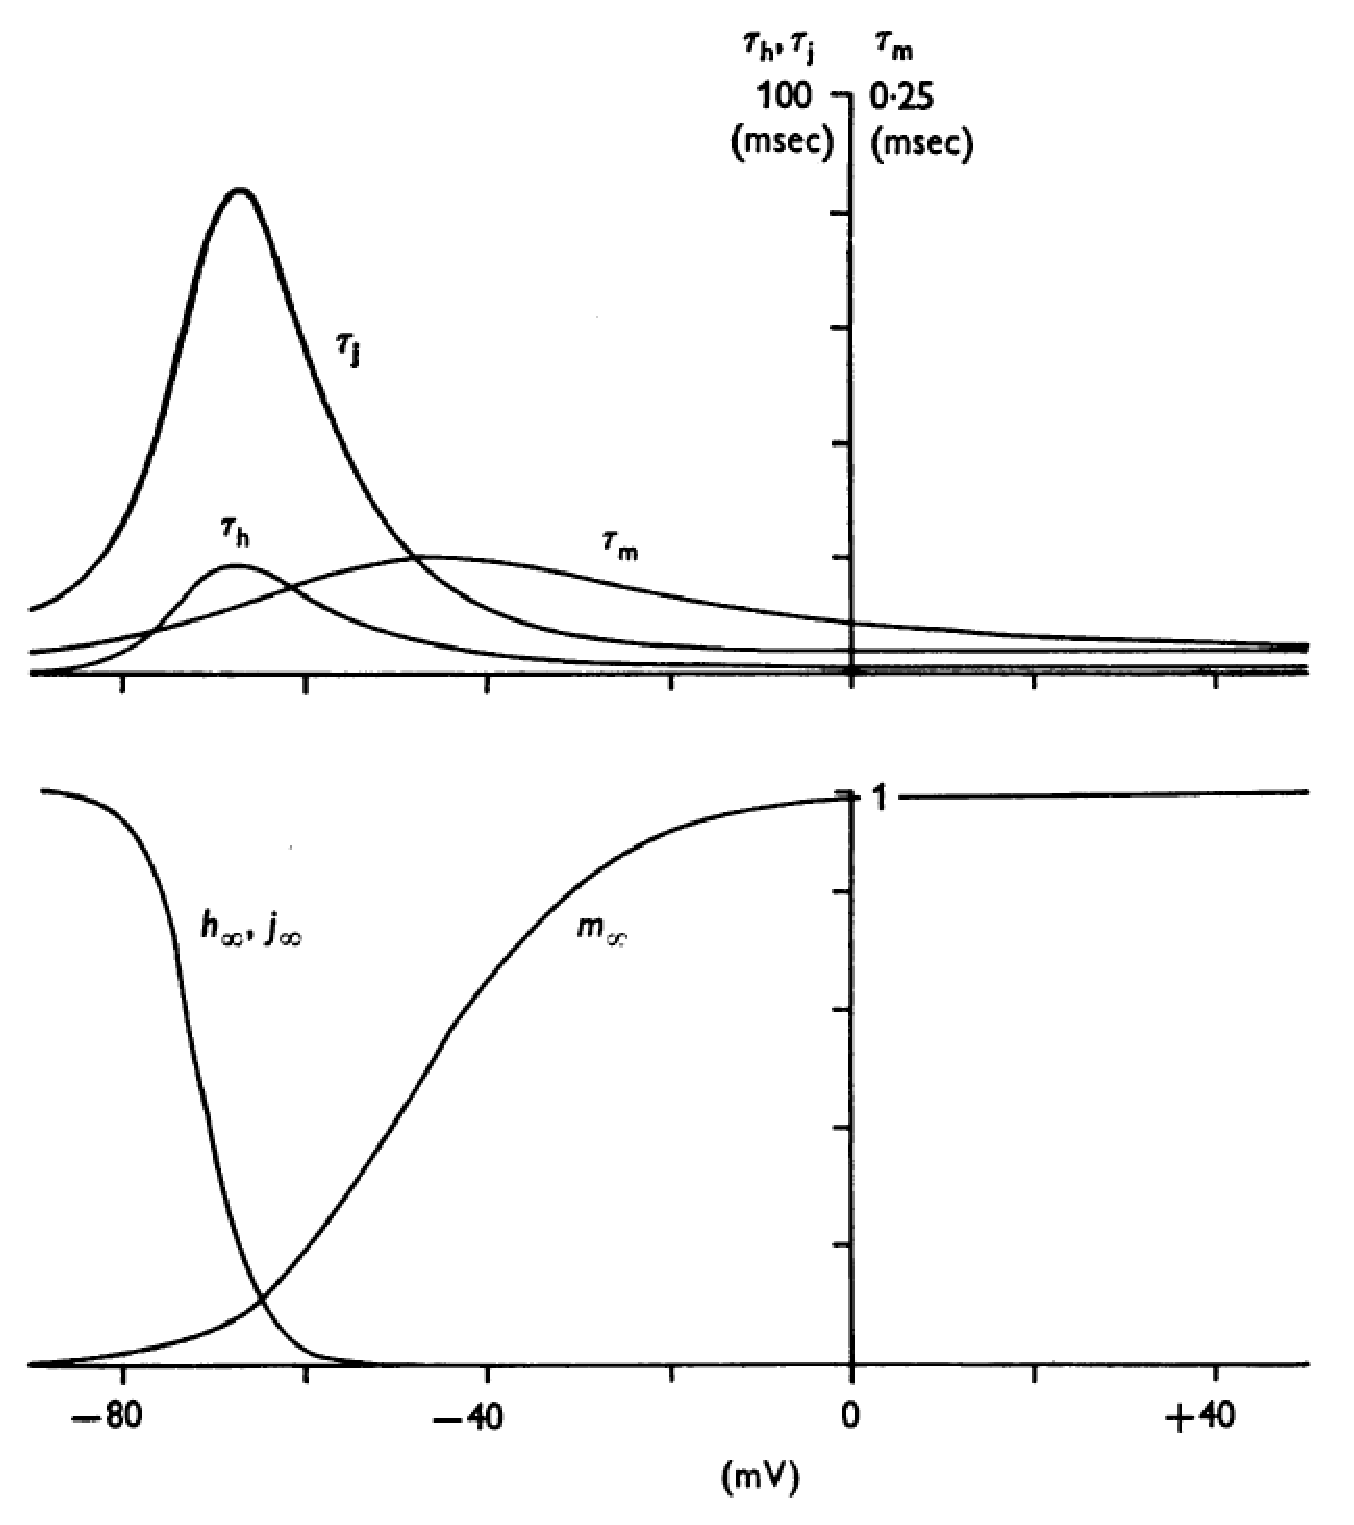
\includegraphics[height=5cm,
%     angle=0]{./images/BR_mhj.eps}}
%   \caption{RyR 4-state model}
%   \label{fig:restrepo_RyR}
% \end{figure}
 

\subsubsection{LCC model}

A single LCC is modeled using 7-state Markov model from \citep{mahajan2008} for
rabbit (Sect.\ref{sec:LCC_Mahajan2008}). The single channel current is modeled using GHK
equation

The changes includes $\overline{c_p}=1.5, \tilde{c_p}=0.5$, and $r_2=6.0$. 

\begin{figure}[hbt]
  \centerline{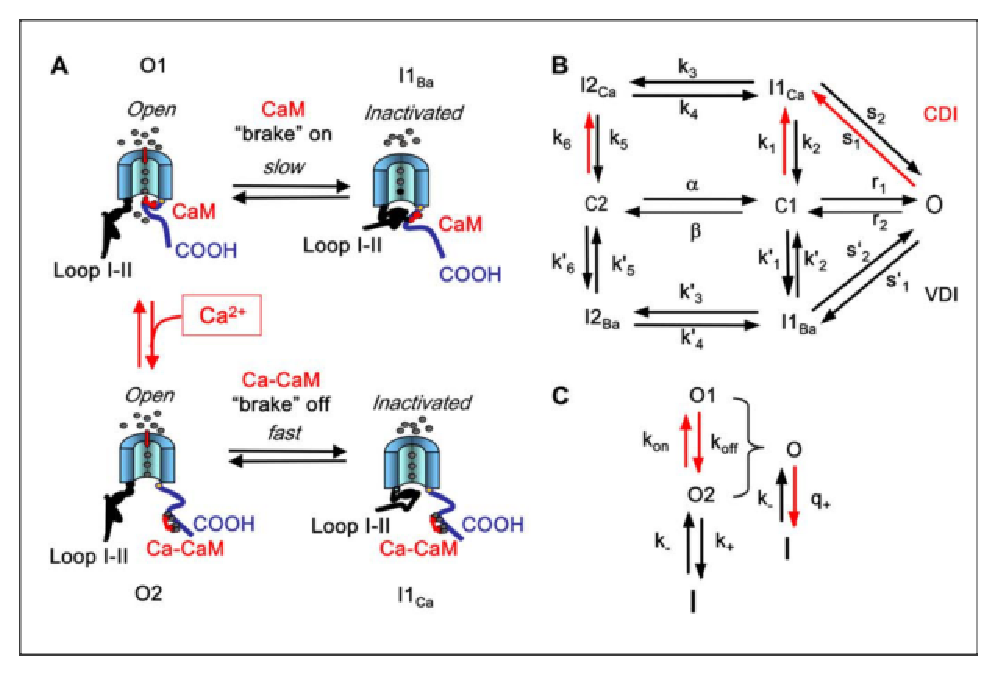
\includegraphics[height=5cm,
    angle=0]{./images/mahajan_LCC.eps}}
  \caption{LCC 7-state model}
  \label{fig:mahajan_LCC}
\end{figure}


\subsection{Diffusion of $\Ca$}

To estime the characteristic time constant for diffusion from one compartment to
another, the formula $\tau \approx \frac{l^2}{D}$. For the case of longitudinal
and transversal CRU separation, they used $l$ as the distance between CRUs. For
the diffusion of calcium on submembrane compartments, 200 nm shorter was used to
take into account the dyadic width 200nm.

CRUs intercalated between Z-planes at the periphery of the myocytes, that may
increase the wave initiation \citep{chen-izu2006tdd, izu2006irr}. To model this,
they incorporated the concept of diffusive coupling.


\begin{framed}
  Under the assumption that all parts of the sarcolemma experience the
  same voltage; other than the membrane voltage $V_m$, there is no
  global variable that couples the CRUs. When the AP is clamped, the
  only influence of one CRU upon the other is the \ce{Ca^2+}
  diffusion.
\end{framed}

\subsection{Bufferings}

Under the assumption that CSQN form dimers only, we have
\begin{equation}
  \label{eq:875}
  \ce{M + M <=>[k_1][k_2] D}
\end{equation}
with $M$ is CSQN in monomer; $D$ is CSQN in dimer;
$k_1([\ce{Ca^2+}]_{JSR}), k_2([\ce{Ca^2+}]_{JSR})$. The transition are
believed to be fast, so we assume the dimers and monomers are in
equilibrium. 

Assumption that only monomeric form of CSQN can bind to T/J complex to 

\subsection{Numerical analysis}

To avoid keeping track of $\sim 20,000 \times 100$ RyRs channels in the myocyte,
they only keep track of the number of channels in each state, e.g. 4 states in
the case of RyRs. This improves the performance by a factor of 20 (from 10RyRs
and 4 LCCs to the number of RyR per state and 4 LCCs). 

The fatest timescale are the diffusions from proximal space to the submembrane
space, and from submembrane space to the cytosol. So, it's assumed that these
processes are in equilibrium and instantaneous.

The fatest of the remaining time scales is the mean open-time of LCC ($\sim 1$
ms), so they used the time step $\Delta t = 0.1$ (ms). They claimed the result
doesn't change when using $\Delta t = 0.02$ (ms). The ODEs were integrated using
explicit Euler method and Markov models were updated after every time step. 


\subsection{Data analysis}

$\Ca$ wave speed in the model is $\sim 85 \mum/s$, which agrees with
experimental values (50$\sim$150 $\mum/s$) \citep{wier1991,williams1992}. 
They concluded that there is no other global variable, except the voltage,
that couples the release sites. When the cell is voltage-clamped, the only
influenece of one release site to another is the passive diffusion of calcium. 

\section{Restrepo-Karma (2009)}
\label{sec:restrepo-karma-2009}


In this first spatial-temporal model of calcium dynamics of cardiac
cells, they addressed a fundamental problem of any model of calcium
release that includes stochasticity and spatial calcium release: 
\begin{itemize}
\item how do individual calcium release units (CRU) maintain the
  coherent pattern of release to produce macroscopic alternations of
  calcium release stable against stochastic dephasing? 
\end{itemize}
They found that coherence is maintained by local coupling through
calcium diffusion or globally by interactions through the membrane
voltage $V_m$. 

\begin{figure}[hbt]
  \centerline{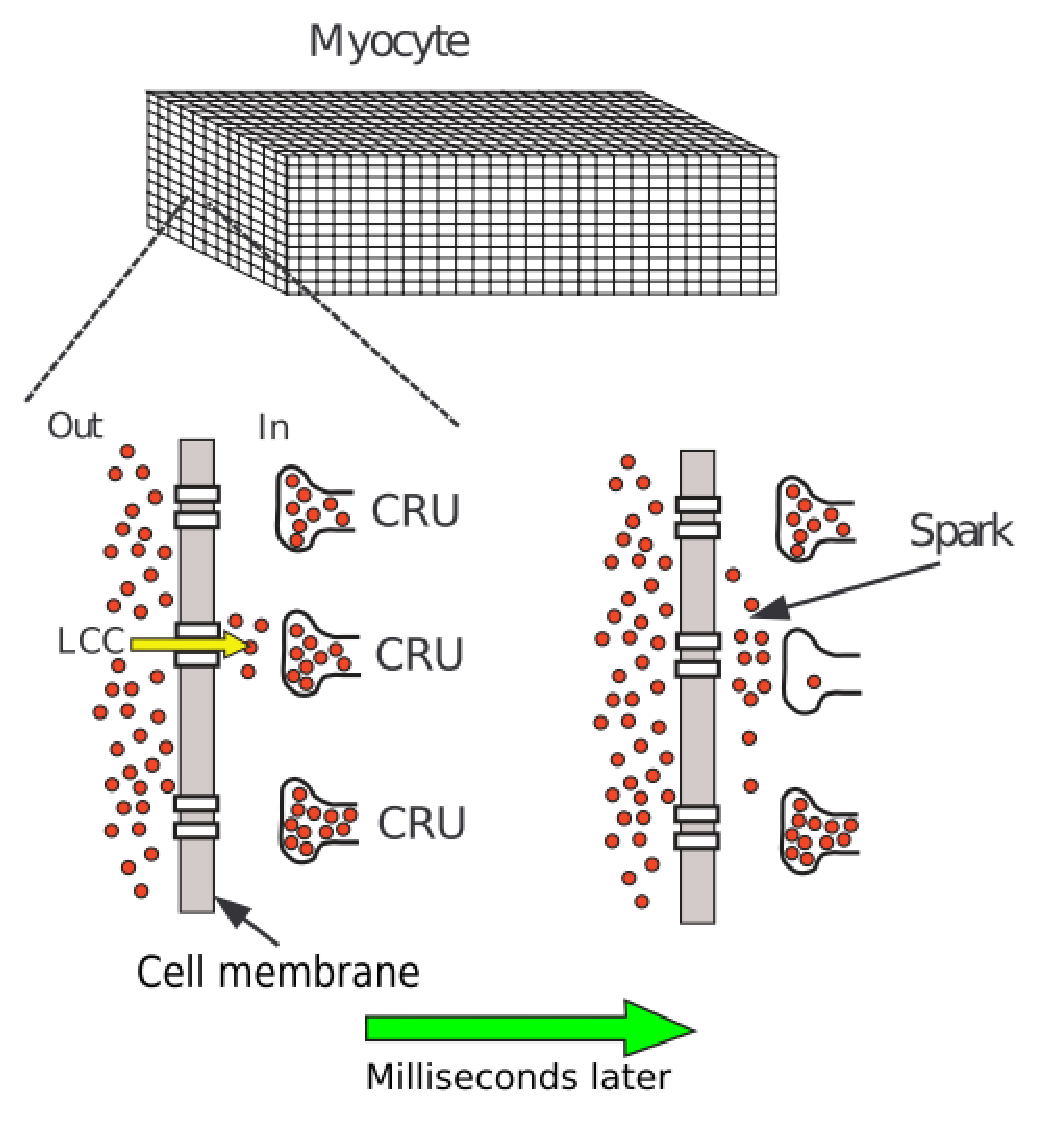
\includegraphics[height=5cm,
    angle=0]{./images/cell_CRU.eps}}
  \caption{Schematic diagram shows 3D grid of a whole-cell with 20,000
    CRUs~\citep{restrepo2009cmc}}
\label{fig:cell_CRU}
\end{figure}

\subsection{Hypothesis analysis}
\label{sec:hypothesis-analysis-7}

\begin{itemize}
\item Number CRU $\sim$ 20,000~\citep{bers2001ecc}
\item A single CRU: few LCC and $\sim$100 RyRs
\item dyadic subspace: $300\times 300\times 15$ nm$^3$
\item junction SR: $300\times 300\times 50$ nm$^3$
\item Inter-CRU distance: 1$\mu$m in the transversal
  direction~\citep{chen-izu2006tdd}, $\sim 2\mu$m in the longitudinal
  direction~\citep{parker1996csi}.
\end{itemize}

The model build a 3D grid of $62\times 32\times12 = 23,808$ grid
elements. In this 3D grid, there are $N=19,305$ CRUs, each modelled
with 14 variables which are concentrations of calcium at different
compartments:
\begin{enumerate}
\item free calcium nsr
\item free calcium jsr
%\item ... myo
\item ... diad subspace (proximal space)
\item ... submembrane space (intermediate the flux between diad
  subspace and myoplasm)
\item (4) number of RyR in one of the 4 states in 4-state Markov-chain
  model
\item (4) state index of each of the 4 LCC
\item (2) calcium bound to Troponin-C in myo and in submembrane
\end{enumerate}





\subsection{Mathematical model}
\label{sec:mathematical-model-12}


\subsubsection{The diffusion}
\label{sec:diffusion-1}


\begin{enumerate}
\item From NSR to JSR: $J_\rf$:
  \begin{equation}
    \label{eq:946}
    J_\rf= v_\rf (c_\nsr - c_\jsr)
  \end{equation}
  with $v_\rf = \frac{1}{\tau_\rf}$. The time constant $\tau_\rf=5$ms
  is chosen so that when taking into account the buffering factor
  $\beta_\jsr\sim 0.15$, the effective refilling time is equal to the
  translocation time from NSR to JSR which is 30ms.


\item From JSR to DS (diad subspace): $J_\ryr$
  \begin{equation}
    \label{eq:948}
    J_\ryr = N_\ryr^o v_\ryr (c_\jsr - c_\ds)
  \end{equation}
with $N_\ryr^o$ is the number of RyR open. 

\item From DS to MYO (myoplasm): $J_\xf$
  \begin{equation}
    \label{eq:947}
    J_\xf= v_\xf (c_\ds - c_\myo)
  \end{equation}
with $v_\xf = \frac{1}{\tau_\xf}$. The time constant
$\tau_\xf=0.222$ms corresponds to the diffusion over a distance of
$\sim 80$nm. 
\end{enumerate}


\section{Nivala et al. (2012)}
\label{sec:nivala2012}

At normal condition, the cluster size of the local transient is the same. Under
the apperance of waves, we then have bigger cluster size which leading to some
cluters is smaller (from the activation of one or a few CRUs), and bigger
clusters (from the activation of many CRUs coupled together). \citep{nivala2012}
applied the idea from \citep{yang2006} to cardiac cells.
Here, power-law distribution applies to spatial clustering and frequency of
fluctuations (both before and after $\Ca$ waves). They claimed that $\Ca$ load
need to be raised to a high enough level for CRUs to be properly coupled and
bring the system to a critical state at which a power-law cluster distribution
exists and $\Ca$ waves start to occur.

As a wave propagates, the SR is emptied, and the system is brought out of the
critical range



%%% Local Variables: 
%%% mode: latex
%%% TeX-master: "document"
%%% End: 